% !TeX root = ../main_ustc.tex
\chapter{基于合作博弈的柔性接触力位协同控制方法}
\label{chap:ch3_force_position_game}

柔性接触操作中，机器人末端工具通常需要沿给定轨迹完成扫描、按压、检测或表面跟随，同时保持接触力处于安全范围。位置目标和力目标在这类任务中紧密耦合。沿切向提高轨迹跟踪精度，有助于保证扫描覆盖和几何路径质量；沿法向维持合适接触力，有助于避免脱离接触、过压或柔性对象损伤。环境刚度、阻尼、接触深度和局部表面形状发生变化时，同样的位置误差可能对应完全不同的接触力响应，固定参数控制器容易在软区和硬区之间出现性能失配。

本章研究给定参考轨迹和期望接触力条件下的执行层控制问题。人类监督输入如何生成或修正参考轨迹，将在第四章作为参考层仲裁问题展开；本章只关注机器人执行给定参考时，如何在位置跟踪和接触力调节之间形成可解释、可实时求解的反馈控制律。为此，本章将位置目标和力目标视为两个共享控制输入的合作参与方，在力位增广状态模型上构造折扣帕累托代价函数，并通过力安全裕度和局部环境刚度估计在线调节力位优先级。

本章使用 $\xi$ 表示柔性接触力位增广状态，使用 $\alpha_{\mathrm{FP}}$ 表示位置目标与力目标之间的优先级。$\alpha_{\mathrm{FP}}$ 数值越大，控制器越偏向位置跟踪；数值越小，控制器越偏向接触力调节。该变量只作用于执行层力位控制，不表示第四章中的人机仲裁权重。

\section{柔性接触任务描述与控制目标}
\label{sec:ch3_problem}

考虑机器人末端携带短探针、圆头工具或长工具尖端与柔性环境保持接触，并沿给定路径执行扫描任务。设 $x(t)\in\R^n$ 为工具接触点位置，$x_d(t)\in\R^n$ 为期望接触轨迹，$f_e(t)\in\R^n$ 为环境作用于工具的接触力，$f_d(t)\in\R^n$ 为期望接触力。柔性环境可以表示为软质工件、橡胶密封件、泡棉材料、仿组织材料或其他具有局部可变刚度的接触对象。任务执行过程中，机器人需要维持连续接触。接触力过大可能造成材料局部损伤或引入较大冲击，接触力过小会降低接触测量和表面跟随的有效性。

为突出接触安全边界，定义受控标量接触力
\begin{equation}
  y_f(t)=S_f f_e(t),
  \label{eq:ch3_yf}
\end{equation}
其中 $S_f\in\R^{1\times n}$ 为力方向选择矩阵。给定安全力范围 $[F_{\min},F_{\max}]$ 和期望力 $F_d$，满足
\begin{equation}
  F_{\min}<F_d<F_{\max}.
  \label{eq:ch3_force_band}
\end{equation}
本章希望 $y_f(t)$ 接近 $F_d$，并尽量保持在安全区间内部。对于切向扫描任务，位置误差主要影响轨迹覆盖和路径质量；对于法向接触任务，位置误差会通过柔性环境刚度放大为接触力误差。力位协同控制的关键在于，控制器需要根据当前接触状态选择合适的折中，使优先级能够随环境条件变化而连续调整。

\begin{problem}[柔性接触力位协同控制问题]
\label{prob:ch3_force_position_control}
考虑机器人末端工具在柔性环境中保持接触并沿期望轨迹运动的任务。给定参考轨迹 $x_d(t)$、期望接触力 $f_d(t)$、安全力范围 $[F_{\min},F_{\max}]$ 以及局部柔性接触模型，设计反馈控制律 $u(t)$ 与力位优先级 $\alpha_{\mathrm{FP}}(t)$，使闭环系统满足以下要求：
\begin{enumerate}[label=(\arabic*)]
  \item 位置误差 $e_p(t)=x(t)-x_d(t)$ 和速度误差 $e_v(t)=\dot x(t)-\dot x_d(t)$ 保持有界并尽量减小；
  \item 力误差 $e_f(t)=f_e(t)-f_d(t)$ 及其稳态偏差得到抑制；
  \item 受控接触力 $y_f(t)$ 尽量保持在 $[F_{\min},F_{\max}]$ 内；
  \item 控制输入满足实时执行要求，优先级变化保持连续和平滑；
  \item 在局部接触模型误差和环境刚度变化存在时，闭环状态仍具有有界性。
\end{enumerate}
\end{problem}

上述问题把本章的研究边界限定在执行层。参考轨迹和期望接触力可以来自离线规划、示教轨迹、任务规划器或后续人机仲裁模块。本章关心的是，在这些参考已经给定的条件下，控制器如何处理轨迹精度、接触力安全和局部环境变化之间的关系。这样安排也使第三章、第四章和第五章形成清晰分工：第三章给出力位控制器，第四章研究人类监督输入进入参考层的方式，第五章在统一平台上验证两层方法组合后的系统表现。

\section{柔性接触力位增广系统建模}
\label{sec:ch3_augmented_model}

柔性接触控制器需要把机器人任务空间运动和环境接触响应写入同一状态模型。第二章已经给出机械臂任务空间建模基础，本节在此基础上建立面向控制器设计的局部等效模型。设工具接触点或等效控制点的任务空间动力学可写为
\begin{equation}
  M_p(q)\ddot x+C_p(q,\dot q)\dot x+G_p(q)=\mu+f_e,
  \label{eq:ch3_task_dynamics}
\end{equation}
其中 $M_p(q)\succ0$ 为任务空间惯性矩阵，$C_p(q,\dot q)$ 为速度相关项，$G_p(q)$ 为重力项，$\mu$ 为机器人任务空间控制输入。实际控制中，内环补偿和局部线性化可将\eqref{eq:ch3_task_dynamics}整理为适合实时反馈设计的修正阻抗模型\cite{hogan1985impedance}：
\begin{equation}
  M\ddot x+C\dot x+K_v(x-x_d)=\mu+f_e,
  \label{eq:ch3_impedance}
\end{equation}
其中 $M\succ0$、$C\succ0$ 和 $K_v\succ0$ 分别为期望惯性、阻尼和基线虚拟刚度矩阵。$K_v$ 提供名义位置恢复作用，使后续力位增广误差模型具有明确的弹性恢复结构。

柔性环境在局部短时间接触区间内采用开尔文--沃伊特模型近似：
\begin{equation}
  f_e=-K_e(x-x_s)-B_e(\dot x-\dot x_s)+\Delta_f(x,\dot x,t),
  \label{eq:ch3_kv_contact}
\end{equation}
其中 $x_s(t)$ 为局部接触面参考位置，$K_e\succeq0$ 和 $B_e\succeq0$ 分别为局部等效刚度与阻尼，$\Delta_f$ 表示材料非线性、摩擦、测量噪声和接触面变化引起的模型误差。该模型服务于局部控制设计，表示扫描过程中接触点附近的表观力学关系。

\begin{assumption}[柔性接触模型局部有效性]
\label{ass:ch3_contact_model}
在每一个短时间接触区间内，柔性环境可由\eqref{eq:ch3_kv_contact}近似描述。矩阵 $K_e$、$B_e$ 以及接触面参考 $x_s(t)$、$\dot x_s(t)$ 在所考虑的紧集内有界。模型误差 $\Delta_f(x,\dot x,t)$ 及其对时间的局部导数有界。
\end{assumption}

真实柔性环境的刚度通常随扫描位置、压入量和材料局部形状变化。为使控制器能够根据环境软硬变化选择反馈增益，本章采用面向增益调度的表观刚度估计。沿受控接触方向定义单向压入量
\begin{equation}
  \delta(t)=\max\{0,x_s(t)-x_n(t)\},
  \label{eq:ch3_delta_contact}
\end{equation}
其中 $x_n(t)$ 为工具尖端在接触法向上的坐标。接触发生后，受控力可近似写为标量开尔文--沃伊特形式
\begin{equation}
  y_f(t)=K_e\delta(t)+B_e\dot\delta(t)+\nu_f(t),
  \label{eq:ch3_scalar_kv}
\end{equation}
其中 $\nu_f(t)$ 汇集测量噪声和未建模接触项。当接触力和压入量足够大时，定义表观刚度观测值
\begin{equation}
  K_{\mathrm{obs}}(t)=
  \sat\left(\frac{|y_f(t)|}{|\delta(t)|},K_{\min},K_{\max}\right),
  \quad |y_f|\ge F_{\mathrm{th}},\ |\delta|\ge\delta_{\min}.
  \label{eq:ch3_K_obs}
\end{equation}
若接触判据尚未满足，则保持上一时刻估计值。刚度估计采用指数低通更新：
\begin{equation}
  \hat K_{e,k}=
  \sat\left(\hat K_{e,k-1}+\alpha_K\left(K_{\mathrm{obs},k}-\hat K_{e,k-1}\right),
  K_{\min},K_{\max}\right),
  \quad 0<\alpha_K<1 .
  \label{eq:ch3_K_ema}
\end{equation}
该估计量用于识别局部软硬变化，并作为离线增益表的调度变量。它不承担精确材料辨识任务，因此采用较稳健的有界低通形式更适合实时控制。

定义位置误差、速度误差和力误差为
\begin{equation}
  e_p=x-x_d,
  \quad e_v=\dot x-\dot x_d,
  \quad e_f=f_e-f_d .
  \label{eq:ch3_errors}
\end{equation}
为减小稳态力误差，引入力误差泄漏积分状态
\begin{equation}
  \dot\sigma_f=e_f-\lambda_f\sigma_f,
  \quad \lambda_f>0 .
  \label{eq:ch3_sigma}
\end{equation}
增广力位误差状态定义为
\begin{equation}
  \xi=\begin{bmatrix}e_p^{\T}&e_v^{\T}&e_f^{\T}&\sigma_f^{\T}\end{bmatrix}^{\T}\in\R^{4n}.
  \label{eq:ch3_xi}
\end{equation}

\begin{assumption}[残差项有界性]
\label{ass:ch3_residual}
将任务空间动力学线性化误差、内环补偿误差、参考轨迹变化、接触面运动、接触模型误差、摩擦、离散化误差和测量噪声统一记为残差项 $d(\xi,t)$。存在非负常数 $\bar d_0$ 与 $\bar d_1$，使得
\begin{equation}
  \norm{d(\xi,t)}\le \bar d_0+\bar d_1\norm{\xi},\quad \forall t\ge0 .
  \label{eq:ch3_residual_bound_affine}
\end{equation}
若只在给定紧集 $\Omega_\xi$ 内分析局部性能，则存在常数 $\bar d>0$，使得
\begin{equation}
  \norm{d(\xi,t)}\le \bar d,
  \quad \xi\in\Omega_\xi .
  \label{eq:ch3_residual_bound_const}
\end{equation}
\end{assumption}

\begin{lemma}[含残差项的增广力位误差系统]
\label{lem:ch3_augmented_system}
在\cref{ass:ch3_contact_model}下，修正阻抗系统\eqref{eq:ch3_impedance}与局部柔性接触模型\eqref{eq:ch3_kv_contact}可写成增广误差系统
\begin{equation}
  \dot\xi=A_c\xi+B_c\mu+d(\xi,t),
  \label{eq:ch3_aug_system_mu}
\end{equation}
其中 $A_c$ 和 $B_c$ 由 $M,C,K_v,K_e,B_e,\lambda_f$ 的局部标称值确定。若采用前馈补偿 $\mu=u_{\mathrm{ff}}+u$，并将未补偿项并入残差，则控制器设计所使用的标称反馈模型为
\begin{equation}
  \dot\xi=A_c\xi+B_cu .
  \label{eq:ch3_nominal_model}
\end{equation}
\end{lemma}

\begin{proof}
由 $e_p=x-x_d$ 可得
\begin{equation}
  \dot e_p=e_v .
  \label{eq:ch3_ep_dot}
\end{equation}
根据修正阻抗动力学\eqref{eq:ch3_impedance}，并代入 $\dot x=e_v+\dot x_d$、$x-x_d=e_p$、$f_e=e_f+f_d$，得到
\begin{equation}
  \dot e_v=-M^{-1}K_ve_p-M^{-1}Ce_v+M^{-1}e_f+M^{-1}\mu+\Delta_v(t),
  \label{eq:ch3_ev_dot}
\end{equation}
其中 $\Delta_v(t)=-M^{-1}C\dot x_d+M^{-1}f_d-\ddot x_d$ 为参考轨迹和期望力引起的仿射项。该项可由前馈输入部分补偿，未补偿部分进入残差。

由 $e_f=f_e-f_d$ 得 $\dot e_f=\dot f_e-\dot f_d$。对\eqref{eq:ch3_kv_contact}求导，并将 $K_e$ 与 $B_e$ 的局部变化归入残差，可得
\begin{equation}
  \dot f_e=-K_e(\dot x-\dot x_s)-B_e(\ddot x-\ddot x_s)+\Delta_{\dot f}(x,\dot x,t).
  \label{eq:ch3_fe_dot}
\end{equation}
将 $\dot x=e_v+\dot x_d$ 以及由\eqref{eq:ch3_impedance}得到的 $\ddot x$ 代入\eqref{eq:ch3_fe_dot}，整理关于 $e_p,e_v,e_f,\mu$ 的项，得到
\begin{equation}
  \dot e_f=B_eM^{-1}K_ve_p+(-K_e+B_eM^{-1}C)e_v-B_eM^{-1}e_f-B_eM^{-1}\mu+\Delta_f^{\mathrm{res}}(\xi,t),
  \label{eq:ch3_ef_dot}
\end{equation}
其中 $\Delta_f^{\mathrm{res}}$ 汇集接触面运动、期望轨迹变化、期望力变化和模型失配项。再由\eqref{eq:ch3_sigma}得到
\begin{equation}
  \dot\sigma_f=e_f-\lambda_f\sigma_f .
  \label{eq:ch3_sigma_dot_final}
\end{equation}
将\eqref{eq:ch3_ep_dot}、\eqref{eq:ch3_ev_dot}、\eqref{eq:ch3_ef_dot}与\eqref{eq:ch3_sigma_dot_final}依次堆叠，即可得到\eqref{eq:ch3_aug_system_mu}。若使用 $\mu=u_{\mathrm{ff}}+u$ 对可计算仿射项进行补偿，剩余反馈设计模型为\eqref{eq:ch3_nominal_model}。引理得证。
\end{proof}

逐轴实现时，可取单轴状态 $\xi_i=[e_{p,i},e_{v,i},e_{f,i},\sigma_{f,i}]^{\T}$，并写成
\begin{equation}
  \dot\xi_i=\bar A_i\xi_i+\bar b_i u_i+d_i(t),
  \label{eq:ch3_axis_state}
\end{equation}
其中
\begin{equation}
  \bar A_i=\begin{bmatrix}
  0&1&0&0\\
  -K_v/M&-C/M&1/M&0\\
  B_eK_v/M&-K_e+B_eC/M&-B_e/M&0\\
  0&0&1&-\lambda_f
  \end{bmatrix},
  \quad
  \bar b_i=\begin{bmatrix}0\\1/M\\-B_e/M\\0\end{bmatrix}.
  \label{eq:ch3_axis_matrices}
\end{equation}
三维任务空间可由逐轴模型按块对角方式扩展。该局部模型是后续合作博弈控制器、离线增益表和在线优先级调节的共同基础。

\section{合作博弈力位协同控制器设计}
\label{sec:ch3_game_controller}

本节将位置跟踪和力调节写成两个合作参与方的折扣代价。两个目标共享同一个控制输入 $u$，因此无法通过互不相关的控制回路分别求解。合作博弈的作用是把位置目标和力目标放入同一个增广系统中，通过帕累托有效解表达柔性接触任务中的动态折中\cite{basar1999dynamic,engwerda2005lqdg}。

\begin{definition}[折扣型位置目标与力目标代价函数]
\label{def:ch3_discount_costs}
对位置跟踪目标和力调节目标，分别定义折扣型无限时域代价函数
\begin{equation}
  J_p(\xi_0,u)=\int_0^\infty \e^{-\gamma t}\left[\xi^{\T}Q_p\xi+u^{\T}R_pu\right]\dd t,
  \label{eq:ch3_Jp}
\end{equation}
\begin{equation}
  J_f(\xi_0,u)=\int_0^\infty \e^{-\gamma t}\left[\xi^{\T}Q_f\xi+u^{\T}R_fu\right]\dd t,
  \label{eq:ch3_Jf}
\end{equation}
其中 $\gamma>0$ 为折扣因子，$Q_p\succeq0$ 主要惩罚 $e_p$ 和 $e_v$，$Q_f\succeq0$ 主要惩罚 $e_f$ 和 $\sigma_f$，$R_p,R_f\succ0$ 为控制输入权重。
\end{definition}

折扣因子使近期误差和近期力风险具有更高权重，也使无限时域代价在存在局部模型近似时更容易用于工程实现。类似的折扣帕累托思路已被用于连续接触任务中的力位协调控制\cite{li2026pareto}。给定力位优先级 $\alpha_{\mathrm{FP}}\in[\alpha_{\min},\alpha_{\max}]\subset(0,1)$，定义
\begin{equation}
  Q_\alpha=\alpha_{\mathrm{FP}}Q_p+\bigl(1-\alpha_{\mathrm{FP}}\bigr)Q_f,
  \label{eq:ch3_Qalpha}
\end{equation}
\begin{equation}
  R_\alpha=\alpha_{\mathrm{FP}}R_p+\bigl(1-\alpha_{\mathrm{FP}}\bigr)R_f .
  \label{eq:ch3_Ralpha}
\end{equation}
对应的标量化折扣代价为
\begin{equation}
  J_\alpha(\xi_0,u)=\int_0^\infty \e^{-\gamma t}\left[\xi^{\T}Q_\alpha\xi+u^{\T}R_\alpha u\right]\dd t .
  \label{eq:ch3_Jalpha}
\end{equation}

\begin{definition}[帕累托有效控制律]
\label{def:ch3_pareto}
若不存在另一个可容许控制律 $\tilde u$，使得 $J_p(\xi_0,\tilde u)\le J_p(\xi_0,u)$ 且 $J_f(\xi_0,\tilde u)\le J_f(\xi_0,u)$，并且至少一个不等式严格成立，则称控制律 $u$ 对双目标代价 $(J_p,J_f)$ 是帕累托有效的。
\end{definition}

在凸二次情形下，加权标量化代价\eqref{eq:ch3_Jalpha}的最优解是支持帕累托解。在线阶段通过调节 $\alpha_{\mathrm{FP}}(t)$，控制器可以在位置跟踪和力调节之间移动工作点。这样，系统无需在每个控制周期重新求解完整多目标优化问题，可利用一个连续优先级选择当前反馈增益。

\begin{assumption}[标称系统可镇定与可检测]
\label{ass:ch3_stabilizable}
标称系统矩阵对 $(A_c,B_c)$ 可镇定。对任意 $\alpha_{\mathrm{FP}}\in[\alpha_{\min},\alpha_{\max}]$，矩阵对 $(Q_\alpha^{1/2},A_c)$ 可检测，并且 $R_\alpha\succ0$。
\end{assumption}

\begin{lemma}[标称系统下的折扣哈密顿--雅可比--贝尔曼方程]
\label{lem:ch3_hjb}
对于标称系统\eqref{eq:ch3_nominal_model}和折扣代价\eqref{eq:ch3_Jalpha}，若 $V_\alpha(\xi)$ 为最优值函数，则其满足折扣哈密顿--雅可比--贝尔曼方程
\begin{equation}
  0=\min_u\left[\xi^{\T}Q_\alpha\xi+u^{\T}R_\alpha u+\nabla V_\alpha^{\T}(A_c\xi+B_cu)-\gamma V_\alpha\right].
  \label{eq:ch3_hjb}
\end{equation}
\end{lemma}

\begin{proof}
由动态规划原理，从任意时刻 $t$ 开始的最优值函数等于当前瞬时代价与后续最优代价之和。对折扣型无限时域问题，在微小时间区间 $[t,t+\Delta t]$ 上展开，有
\begin{align}
  V_\alpha(\xi(t))=&\min_u\int_t^{t+\Delta t}\e^{-\gamma(\tau-t)}\ell_\alpha(\xi(\tau),u(\tau))\dd\tau \\
  &+\e^{-\gamma\Delta t}V_\alpha(\xi(t+\Delta t)),
\end{align}
其中 $\ell_\alpha(\xi,u)=\xi^{\T}Q_\alpha\xi+u^{\T}R_\alpha u$。对 $V_\alpha(\xi(t+\Delta t))$ 作一阶展开，并令 $\Delta t$ 趋近于零，整理可得\eqref{eq:ch3_hjb}。引理得证。
\end{proof}

\begin{theorem}[固定力位优先级下的折扣帕累托反馈律]
\label{thm:ch3_discount_lqr}
在\cref{ass:ch3_stabilizable}成立的条件下，给定固定 $\alpha_{\mathrm{FP}}\in[\alpha_{\min},\alpha_{\max}]$。若 $P_\alpha=P_\alpha^{\T}\succeq0$ 是折扣代数黎卡提方程
\begin{equation}
  A_c^{\T}P_\alpha+P_\alpha A_c-P_\alpha B_cR_\alpha^{-1}B_c^{\T}P_\alpha+Q_\alpha-\gamma P_\alpha=0
  \label{eq:ch3_discount_are}
\end{equation}
的稳定化解，则折扣标量化代价\eqref{eq:ch3_Jalpha}对应的最优反馈律为
\begin{equation}
  u_\alpha^*(\xi)=-R_\alpha^{-1}B_c^{\T}P_\alpha\xi .
  \label{eq:ch3_u_star}
\end{equation}
\end{theorem}

\begin{proof}
设二次型值函数为 $V_\alpha(\xi)=\xi^{\T}P_\alpha\xi$，则 $\nabla V_\alpha=2P_\alpha\xi$。将其代入\eqref{eq:ch3_hjb}中的哈密顿函数，得到
\begin{equation}
  \mathcal{H}_\alpha(\xi,u)=\xi^{\T}Q_\alpha\xi+u^{\T}R_\alpha u+2\xi^{\T}P_\alpha A_c\xi+2\xi^{\T}P_\alpha B_cu-\gamma\xi^{\T}P_\alpha\xi .
\end{equation}
对 $u$ 求偏导，有
\begin{equation}
  \frac{\partial\mathcal{H}_\alpha}{\partial u}=2R_\alpha u+2B_c^{\T}P_\alpha\xi .
\end{equation}
由 $R_\alpha\succ0$ 可知哈密顿函数关于 $u$ 严格凸。令偏导为零，得到唯一极小点\eqref{eq:ch3_u_star}。将该控制律代回\eqref{eq:ch3_hjb}，得到
\begin{equation}
  \xi^{\T}\left[A_c^{\T}P_\alpha+P_\alpha A_c-P_\alpha B_cR_\alpha^{-1}B_c^{\T}P_\alpha+Q_\alpha-\gamma P_\alpha\right]\xi=0 .
\end{equation}
由于该式对任意 $\xi$ 成立，括号中的矩阵为零，因此 $P_\alpha$ 满足\eqref{eq:ch3_discount_are}。定理得证。
\end{proof}

为了满足接触控制的实时性要求，反馈增益采用离线表和在线插值实现。离线阶段在 $\alpha_{\mathrm{FP}}$ 与局部刚度估计 $\hat K_e$ 的二维网格上求解\eqref{eq:ch3_discount_are}，得到增益表
\begin{equation}
  K(\alpha_{\mathrm{FP}},\hat K_e)=R_\alpha^{-1}B_c^{\T}P_\alpha .
  \label{eq:ch3_gain_table}
\end{equation}
在线阶段只更新 $\alpha_{\mathrm{FP}}(t)$ 和 $\hat K_e(t)$，并通过插值得到当前反馈增益。控制输入写为
\begin{equation}
  u(t)=-K(\alpha_{\mathrm{FP}}(t),\hat K_e(t))\xi(t).
  \label{eq:ch3_control_law}
\end{equation}
这种离线--在线结构将控制器求解、环境估计和优先级调节分开处理。控制器给出每个候选优先级与局部刚度下的最优反馈律，环境估计器提供当前表观刚度，优先级调节模块根据接触安全状态选择合适的折中点。

\section{力安全裕度与动态优先级调节}
\label{sec:ch3_priority}

折扣帕累托控制器给出了可调优先级下的力位反馈律，接下来需要说明 $\alpha_{\mathrm{FP}}(t)$ 如何在线选择。刚度反映环境属性，接触力安全裕度反映当前控制风险。二者结合可以使优先级既响应力边界，又体现软硬材料变化对压入敏感性的影响。

\begin{definition}[接触力安全裕度]
\label{def:ch3_force_margin}
给定受控力 $y_f(t)$ 和安全范围 $[F_{\min},F_{\max}]$，定义到下界和上界的距离为
\begin{equation}
  d_{\mathrm{lower}}(t)=y_f(t)-F_{\min},
  \quad d_{\mathrm{upper}}(t)=F_{\max}-y_f(t) .
  \label{eq:ch3_force_distances}
\end{equation}
归一化安全裕度定义为
\begin{equation}
  \rho_F(t)=\sat\left(\frac{\min\{d_{\mathrm{lower}}(t),d_{\mathrm{upper}}(t)\}}{(F_{\max}-F_{\min})/2},0,1\right) .
  \label{eq:ch3_rhoF}
\end{equation}
边界方向变量定义为
\begin{equation}
  s_F(t)=\sat\left(\frac{y_f(t)-F_d}{(F_{\max}-F_{\min})/2},-1,1\right) .
  \label{eq:ch3_sF}
\end{equation}
其中 $\rho_F(t)$ 越接近 $1$，表示接触力越接近安全区间中部；越接近 $0$，表示接触力越接近上下边界。$s_F(t)>0$ 表示接触力偏大，$s_F(t)<0$ 表示接触力偏小。
\end{definition}

执行层优先级调节只使用机器人状态、接触力和环境估计量，不使用主端输入、操作者意图或目标切换信息，因此它与第四章的人机仲裁权重 $\alpha_{\mathrm{HR}}$ 保持分离。对于表面扫描任务，切向位置误差主要决定路径覆盖，法向位置误差直接改变压入深度和接触力。实际实现中可采用逐轴优先级
\begin{equation}
  \boldsymbol{\alpha}_{\mathrm{FP}}(t)
  =
  \begin{bmatrix}
  1 & 1 & \alpha_z(t)
  \end{bmatrix}^{\T},
  \label{eq:ch3_axis_alpha}
\end{equation}
使切向 $x$ 和 $y$ 方向保持位置主导，法向 $z$ 方向通过 $\alpha_z$ 在压入深度稳定与接触力调节之间切换。若任务三轴均存在接触力耦合，也可令三个方向分别采用独立的 $\alpha_i(t)$。下文为简洁起见仍以 $\alpha_{\mathrm{FP}}$ 表示当前需要调节的执行层优先级。

在接触开始、稳定扫描和退回阶段，力误差的物理含义存在差异。为避免刚接触瞬态直接驱动优先级突变，引入连续阶段先验。设 $F_{\mathrm{th}}$ 为接触检测阈值，$t_c$ 为连续接触时间，$\dot z$ 为法向速度。定义
\begin{equation}
  c_F=\sigma\left(\frac{|y_f|-F_{\mathrm{th}}}{b_F}\right),
  \quad
  c_v=\sigma\left(\frac{-\dot z-\dot z_{\mathrm{th}}}{b_v}\right),
  \quad
  c_t=S\left(\frac{t_c}{T_{\mathrm{trans}}}\right),
  \label{eq:ch3_phase_gates}
\end{equation}
其中 $\sigma(\cdot)$ 为 Sigmoid 函数，$S(q)=q^2(3-2q)$ 为平滑阶跃函数，$b_F$、$b_v$ 和 $T_{\mathrm{trans}}$ 为正常数。自由空间与接近阶段先验、接触瞬态与稳定阶段先验分别写为
\begin{equation}
  \alpha_{\mathrm{pre}}=(1-c_v)\alpha_{\mathrm{free}}+c_v\alpha_{\mathrm{app}},
  \quad
  w_{\mathrm{pre}}=(1-c_v)w_{\mathrm{free}}+c_vw_{\mathrm{app}},
  \label{eq:ch3_phase_pre}
\end{equation}
\begin{equation}
  \alpha_{\mathrm{con}}=(1-c_t)\alpha_{\mathrm{trans}}+c_t\alpha_{\mathrm{steady}},
  \quad
  w_{\mathrm{con}}=(1-c_t)w_{\mathrm{trans}}+c_tw_{\mathrm{steady}} .
  \label{eq:ch3_phase_contact}
\end{equation}
连续阶段先验为
\begin{equation}
  \alpha_\phi=(1-c_F)\alpha_{\mathrm{pre}}+c_F\alpha_{\mathrm{con}},
  \quad
  w_\phi=(1-c_F)w_{\mathrm{pre}}+c_Fw_{\mathrm{con}} .
  \label{eq:ch3_phase_prior}
\end{equation}
其中 $w_\phi\in[0,1]$ 表示阶段先验对最终优先级的影响程度。自由空间和退回阶段通常取较大的 $w_\phi$，使控制器保持位置主导；稳定接触后逐步降低 $w_\phi$，让力安全裕度和局部刚度主导优先级调节。

在稳定接触阶段，基础优先级采用力安全裕度模糊推理生成。令
\begin{equation}
  W_F=F_{\max}-F_{\min},
  \quad H_F=\frac{W_F}{2},
  \quad e_F=y_f-F_d .
  \label{eq:ch3_force_width}
\end{equation}
构造三个模糊输入：
\begin{equation}
  F_h=\sat\left(\frac{2|e_F|}{W_F},0,2\right),
  \quad
  S_h=6\rho_F,
  \quad
  D_p=\sat\left(D_{\max}-k_p\norm{e_p},0,D_{\max}\right).
  \label{eq:ch3_fuzzy_inputs}
\end{equation}
其中 $F_h$ 描述力误差幅值，$S_h$ 描述接触力距离安全边界的裕度，$D_p$ 描述位置误差是否已经明显增大。$D_p$ 采用反向定义：位置误差较小时 $D_p$ 较大，位置误差较大时 $D_p$ 较小。三类输入分别划分为 $\{\mathrm{PS},\mathrm{PM},\mathrm{PL}\}$ 三个语言变量，输出 $\alpha_0$ 划分为 $\{\mathrm{Z},\mathrm{PS},\mathrm{PM},\mathrm{P},\mathrm{PL}\}$ 五个语言变量。隶属函数采用三角形函数与左右肩函数组合，以保证边界处输出连续。

模糊逻辑控制器的输入、输出和物理趋势可以按如下方式理解。输入端的 $F_h$ 越大，表示当前接触力偏离期望力越明显；若此时位置误差较小，即 $D_p$ 较大，控制器可以降低 $\alpha_0$，让力误差项和力积分项在合作博弈代价中占更大比例。输入端的 $S_h$ 越小，表示接触力越接近安全边界，模糊规则倾向于输出中等或较大的 $\alpha_0$，为后续上边界保护和法向稳定留出余量。输入端的 $D_p$ 越小，表示位置误差越大，规则输出整体向 $\mathrm{P}$ 或 $\mathrm{PL}$ 移动，使控制器优先恢复轨迹或压入深度稳定。输出端的 $\alpha_0$ 是未经方向修正的基础优先级，数值越大表示位置目标权重越高，数值越小表示力目标权重越高。

三类输入的尺度参数会直接改变模糊控制器的灵敏度。安全力区间宽度 $W_F$ 增大时，同样的力偏差对应更小的 $F_h$，控制器对力误差的响应更温和；$W_F$ 缩小时，同样的力偏差更容易进入 $\mathrm{PM}$ 或 $\mathrm{PL}$ 区域。$D_{\max}$ 和 $k_p$ 决定位置误差到 $D_p$ 的映射斜率，$k_p$ 越大，较小位置误差也会使 $D_p$ 快速下降，从而更早提高位置优先级。输出隶属函数的中心位置决定 $\alpha_0$ 的实际数值范围，例如 $\mathrm{Z}$ 对应强力调节，$\mathrm{PM}$ 对应折中优先级，$\mathrm{PL}$ 对应强位置保持。

\begin{figure}[htbp]
  \centering
  \begin{minipage}[t]{0.58\textwidth}
    \centering
    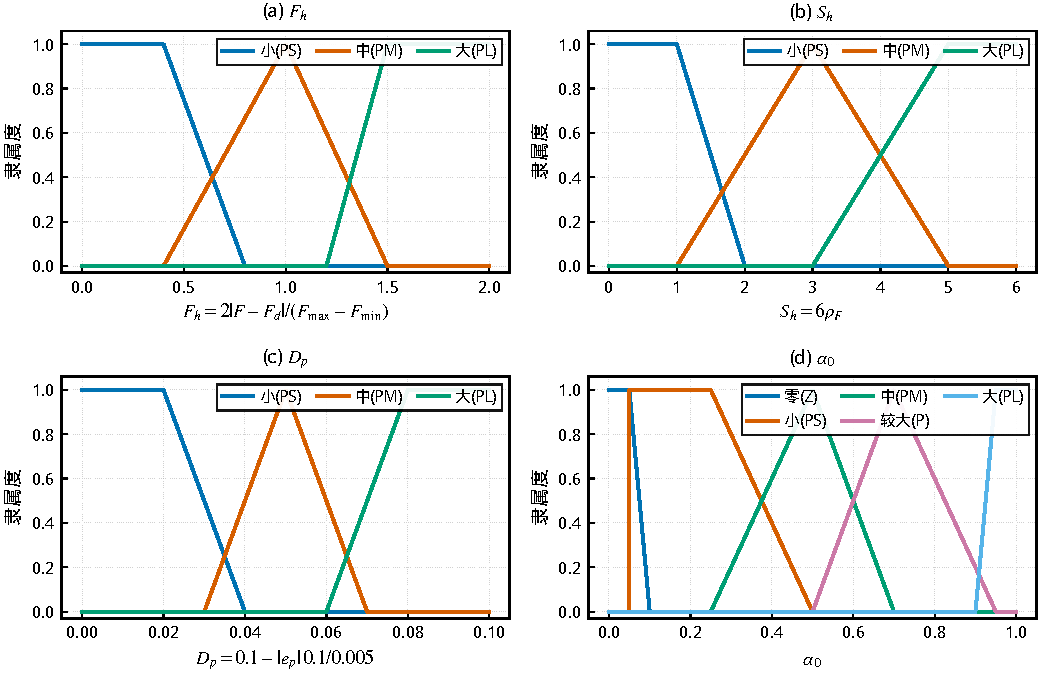
\includegraphics[width=\linewidth]{figures/ch3/ch3_force_margin_membership_ieee.pdf}
  \end{minipage}\hfill
  \begin{minipage}[t]{0.39\textwidth}
    \centering
    
\includegraphics[width=\linewidth]{figures/ch3/ch3_force_margin_surface_ieee.pdf}
  \end{minipage}
  \caption{力安全裕度模糊仲裁器的隶属函数与基础控制曲面。}
  \label{fig:ch3_force_margin_fis}
\end{figure}

图\ref{fig:ch3_force_margin_fis}给出了力安全裕度模糊仲裁器的隶属函数和基础控制曲面。左侧四个子图分别对应 $F_h$、$S_h$、$D_p$ 和 $\alpha_0$ 的语言变量划分。$F_h$ 由当前力误差归一化得到，曲线中“小”“中”“大”三个语言集重叠，使力误差从轻微偏差过渡到明显偏差时不会产生离散跳变。$S_h$ 与安全裕度 $\rho_F$ 成正比，$S_h$ 较小说明接触力接近上下边界，因此低裕度区域会更容易激活保守规则。$D_p$ 采用反向位置裕度定义，位置误差较大时 $D_p$ 落入“小”区域，规则库倾向于提高位置优先级；位置误差较小时 $D_p$ 落入“大”区域，控制器可以释放更多力调节能力。输出端 $\alpha_0$ 采用五个语言集，覆盖从强力调节到强位置保持的连续区间。

图\ref{fig:ch3_force_margin_fis}右侧为固定 $S_h=6$ 时的基础控制曲面，用于展示 $F_h$ 和 $D_p$ 对 $\alpha_0$ 的共同影响。曲面高值区域对应位置优先，低值区域对应力优先。当 $D_p$ 较小时，位置误差已经较大，曲面整体保持较高的 $\alpha_0$，使系统优先恢复轨迹或压入深度稳定。当 $D_p$ 较大且 $F_h$ 增大时，曲面向低值区域下降，说明在位置状态允许的条件下，控制器会降低位置权重并增强力误差修正。曲面中间的平滑过渡来自隶属函数重叠与重心解模糊，体现了模糊控制器将规则表转化为连续仲裁参数的过程。

模糊规则库围绕三个原则构造。第一，当 $D_p$ 较小时，说明位置误差已经明显增大，无论力误差 $F_h$ 处于小、中还是大，输出均偏向 $\mathrm{P}$ 或 $\mathrm{PL}$，使基础优先级 $\alpha_0$ 提高，从而优先恢复轨迹或压入深度稳定。第二，当 $D_p$ 较大且 $F_h$ 较大时，说明位置状态仍可接受而力误差需要修正，输出向 $\mathrm{Z}$ 或 $\mathrm{PS}$ 移动，使控制器释放更多力调节能力。第三，当安全裕度 $S_h$ 较小时，规则整体更保守；即使力误差本身不大，也不让 $\alpha_0$ 过低，以便为后续方向安全修正和边界保护预留稳定裕度。处于中间区域的规则输出 $\mathrm{PS}$、$\mathrm{PM}$ 或 $\mathrm{P}$，用于在位置恢复和力误差修正之间形成平滑过渡。

各参数对模糊优先级的影响也可以直接从上述规则理解。$F_h$ 增大表示力误差幅值增大：若 $D_p$ 较大，$\alpha_0$ 会下降，控制器更偏力调节；若 $D_p$ 较小，位置误差已经不可忽略，规则仍保持较高位置优先级。$S_h$ 增大表示接触力距离安全边界更远，优先级可以更多由 $F_h$ 和 $D_p$ 决定；$S_h$ 减小时，规则输出更保守。$D_p$ 增大表示位置误差较小，允许降低 $\alpha_0$ 以修正力误差；$D_p$ 降低表示位置误差变大，会更早触发位置优先。安全力区间宽度 $W_F$ 增大时，同样的力误差对应更小的 $F_h$，模糊控制器对力误差的响应更温和；位置误差映射增益 $k_p$ 增大时，较小位置误差即可使 $D_p$ 下降，从而提前提高位置优先级。输出隶属函数中心整体右移时，同一组规则激活下得到更大的 $\alpha_0$，闭环更偏位置保持。方向修正参数 $k_{\mathrm{upper}}$ 和 $k_{\mathrm{lower}}$ 不改变基础模糊规则，但会分别增强高力侧和低力侧的安全修正：前者在接触力偏大且裕度下降时更快提高 $\alpha_{\mathrm{FP}}$，后者在接触力偏小时更快降低 $\alpha_{\mathrm{FP}}$，以增强接触力恢复。

设 $\mu_A^F$、$\mu_B^S$ 和 $\mu_C^D$ 分别为输入隶属度。对规则 $(A,B,C)\mapsto Y$，采用 Mamdani 最小激活：
\begin{equation}
  \omega_{ABC}=\min\{\mu_A^F(F_h),\mu_B^S(S_h),\mu_C^D(D_p)\}.
  \label{eq:ch3_fuzzy_activation}
\end{equation}
同一输出标签的激活度采用最大合成。设合成后的输出隶属函数为 $\mu_{\alpha}(z)$，则基础模糊优先级由重心法得到：
\begin{equation}
  \alpha_0=
  \frac{\int_0^1 z\mu_{\alpha}(z)\dd z}
       {\int_0^1 \mu_{\alpha}(z)\dd z}.
  \label{eq:ch3_alpha0}
\end{equation}
若分母过小，则取 $\alpha_0=0.5$ 作为中性优先级。

模糊推理得到的 $\alpha_0$ 主要反映误差幅值和安全裕度，仍需要利用 $s_F$ 区分上边界风险和下边界风险。定义风险强度 $r_F(t)=1-\rho_F(t)$，采用带方向的安全修正：
\begin{equation}
  \alpha_{\mathrm{FM}}(t)=
  \alpha_0(t)+k_{\mathrm{upper}}r_F(t)\max\{s_F(t),0\}
  -k_{\mathrm{lower}}r_F(t)\max\{-s_F(t),0\},
  \label{eq:ch3_alpha_fm}
\end{equation}
其中 $k_{\mathrm{upper}}>0$ 与 $k_{\mathrm{lower}}>0$ 为修正系数。$s_F>0$ 表示接触力偏大，可提高 $\alpha_{\mathrm{FP}}$，使法向位置恢复或几何稳定项占比增加，从而抑制继续压入和振荡；$s_F<0$ 表示接触力偏小，可降低 $\alpha_{\mathrm{FP}}$，使控制器更重视力调节和接触恢复。工程实现中还可加入边界保护
\begin{equation}
  y_f\ge F_{\max}\Rightarrow
  \alpha_{\mathrm{FM}}\leftarrow\max\{\alpha_{\mathrm{FM}},\alpha_{\mathrm{up}}\},
  \quad
  y_f\le F_{\min}\Rightarrow
  \alpha_{\mathrm{FM}}\leftarrow\min\{\alpha_{\mathrm{FM}},\alpha_{\mathrm{low}}\}.
  \label{eq:ch3_alpha_guard}
\end{equation}

在安全裕度充足且力误差较小时，如果位置误差仍持续存在，优先级应适度回到位置主导，避免为了追求力误差而牺牲扫描覆盖。定义安全跟踪门控
\begin{equation}
  \eta_T=
  S\left(\frac{\rho_F-\rho_s}{\rho_1-\rho_s}\right)
  \left[1-S\left(\frac{|e_F|-\varepsilon_F^0}{\varepsilon_F^1-\varepsilon_F^0}\right)\right]
  S\left(\frac{\norm{e_p}-\varepsilon_p^0}{\varepsilon_p^1-\varepsilon_p^0}\right),
  \label{eq:ch3_safe_tracking_gate}
\end{equation}
并令
\begin{equation}
  \alpha_{\mathrm{ST}}=
  \alpha_{\mathrm{FM}}+\eta_T\max\{0,\alpha_{\mathrm{trk}}-\alpha_{\mathrm{FM}}\}.
  \label{eq:ch3_alpha_safe_tracking}
\end{equation}
其中 $0\le\eta_T\le1$，$\rho_s<\rho_1$，$\varepsilon_F^0<\varepsilon_F^1$，$\varepsilon_p^0<\varepsilon_p^1$。该项只在“力安全、力误差小、位置误差仍需修正”时生效，因此不会削弱边界风险下的力安全调节。

\begin{figure}[htbp]
  \centering
  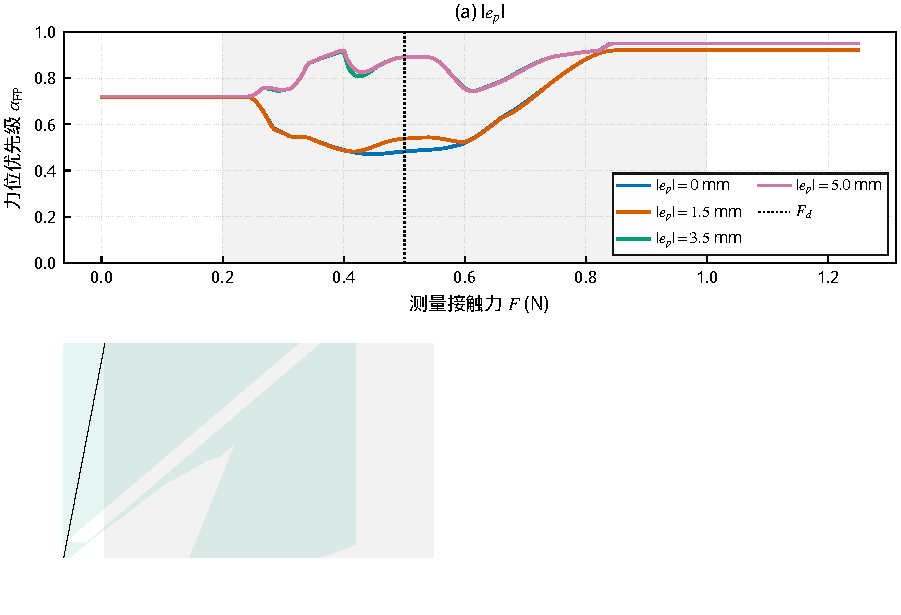
\includegraphics[width=0.96\textwidth]{figures/ch3/ch3_force_margin_trends_ieee.pdf}
  \caption{力安全裕度模糊仲裁器的参数趋势。}
  \label{fig:ch3_force_margin_trends}
\end{figure}

图\ref{fig:ch3_force_margin_trends}进一步展示方向修正和安全跟踪项对优先级的影响，图中灰色区域表示安全力区间，竖直虚线表示期望接触力 $F_d$。图(a)固定力安全边界和模糊规则，仅改变位置误差幅值。位置误差较小时，接触力接近期望值附近的优先级可以降至较低水平，控制器有较大空间修正力误差；随着 $|e_p|$ 增大，安全跟踪门控逐渐生效，曲线整体上移，表示系统在力仍处于安全区间时主动提高位置优先级，以避免扫描轨迹偏离或压入深度漂移。图(b)和图(c)固定 $|e_p|=1.5\,\mathrm{mm}$，分别放大下边界增益和上边界增益的有效作用区间。这样绘制的原因在于方向修正项具有单侧性：$k_{\mathrm{lower}}$ 只通过 $r_F\max\{-s_F,0\}$ 作用于 $F<F_d$ 的低力侧，$k_{\mathrm{upper}}$ 只通过 $r_F\max\{s_F,0\}$ 作用于 $F>F_d$ 的高力侧。若将两者放在全力域同一坐标轴上比较，增大 $k_{\mathrm{lower}}$ 后的曲线在高力侧与默认参数曲线重合是公式结构导致的必然结果，而不是参数失效。因此，图(b)只展示低力侧差异，图(c)只展示高力侧差异，以突出两个方向增益各自的调节含义。

图\ref{fig:ch3_force_margin_trends}(a)中的局部峰谷来自三类机制的叠加。首先，在低接触力区域，低力边界保护使优先级保持在中高水平，避免未形成稳定接触时过度依赖力误差造成继续压入。随后进入安全力区间后，若 $|e_p|$ 较小，模糊规则允许 $\alpha_{\mathrm{FP}}$ 在 $F_d$ 附近形成低谷，将更多控制能力分配给力误差修正；该低谷对应“位置状态可接受、力误差需要修正”的工况。若 $|e_p|$ 增大，安全跟踪门控 $\eta_T$ 在力裕度充足且力误差较小时激活，于是曲线在安全区间中部形成波峰，表示控制器主动恢复位置跟踪。继续向较大接触力方向移动时，上边界风险逐渐增大，方向修正项抬高优先级，因此曲线在靠近上边界时再次上升，体现了抑制过压和法向振荡的需求。中间的小幅波谷则对应 $F_h$、$S_h$、$D_p$ 隶属度交叠区内规则后件的切换，经过一阶滤波进入真实控制后会进一步变得平滑。

图\ref{fig:ch3_force_margin_trends}(b)中，增大 $k_{\mathrm{lower}}$ 后曲线在低力侧相对默认参数明显下降，表示当测量力低于期望值且接近下边界时，控制器主动降低 $\alpha_{\mathrm{FM}}$，给力调节项更大的权重以恢复接触力。随着接触力向 $F_d$ 靠近，$|s_F|$ 减小，下边界方向修正逐步消失，两条曲线自然汇合。低力端出现的平台来自 $\alpha_{\min}$ 饱和和下边界风险限制，说明控制器不会无限降低位置优先级。图(c)中，增大 $k_{\mathrm{upper}}$ 后曲线在高力侧被抬高，表示当接触力高于期望值且向上边界靠近时，控制器更偏向位置恢复和卸载趋势。高力端曲线在峰值后出现平台或轻微回落，是由于 $F_h$、$s_F$ 和 $\rho_F$ 在边界附近进入饱和区，模糊输出不再随力继续线性增长；实际执行时还会叠加边界保护和一阶滤波，使最终 $\alpha_{\mathrm{FP}}$ 保持有界且连续。

为了体现局部环境软硬变化，引入刚度门控函数
\begin{equation}
  g_K(t)=S\left(\frac{\hat K_e(t)-K_{\mathrm{low}}}{K_{\mathrm{high}}-K_{\mathrm{low}}}\right),
  \quad
  S(q)=q^2(3-2q),\ q\in[0,1],
  \label{eq:ch3_gK}
\end{equation}
以及刚度目标优先级
\begin{equation}
  \alpha_K(t)=\bigl(1-g_K(t)\bigr)\alpha_{K,\mathrm{low}}+g_K(t)\alpha_{K,\mathrm{high}} .
  \label{eq:ch3_alphaK}
\end{equation}
其中 $\alpha_{K,\mathrm{low}}$ 与 $\alpha_{K,\mathrm{high}}$ 由任务的法向参考含义确定。若高刚度区的主要风险来自压入深度微小偏差和振荡，可取 $\alpha_{K,\mathrm{high}}>\alpha_{K,\mathrm{low}}$，增强法向位置恢复；若高刚度区采用显式卸载参考，则可取相反设置，使控制器更偏力调节。本文后续实验采用前一种设定，与逐轴扫描控制中法向参考固定、切向严格跟踪的实现一致。

将力安全模糊输出、安全跟踪项、刚度响应项和阶段先验融合，得到目标优先级
\begin{equation}
  \alpha_r(t)=
  \sat\left(
  w_\phi(t)\alpha_\phi(t)
  +\bigl(1-w_\phi(t)\bigr)
  \left[(1-\beta_K)\alpha_{\mathrm{ST}}(t)+\beta_K\alpha_K(t)\right],
  \alpha_{\min},\alpha_{\max}
  \right),
  \label{eq:ch3_alpha_r}
\end{equation}
其中 $\beta_K\in[0,1]$ 表示刚度响应项权重。最终执行的力位优先级由一阶滤波得到：
\begin{equation}
  \dot\alpha_{\mathrm{FP}}(t)=\lambda_{\alpha}(\alpha_r(t)-\alpha_{\mathrm{FP}}(t)),\quad \lambda_\alpha>0 .
  \label{eq:ch3_alpha_ode}
\end{equation}
滤波环节使优先级连续变化，降低瞬时力噪声、刚接触瞬态和模糊规则切换对反馈增益的直接冲击。

\begin{lemma}[力位优先级的区间不变性与变化率上界]
\label{lem:ch3_alpha_bound}
若 $\alpha_{\mathrm{FP}}(0)\in[\alpha_{\min},\alpha_{\max}]$，且 $\alpha_r(t)\in[\alpha_{\min},\alpha_{\max}]$，则\eqref{eq:ch3_alpha_ode}生成的 $\alpha_{\mathrm{FP}}(t)$ 满足
\begin{equation}
  \alpha_{\mathrm{FP}}(t)\in[\alpha_{\min},\alpha_{\max}],\quad \forall t\ge0,
  \label{eq:ch3_alpha_interval}
\end{equation}
并且
\begin{equation}
  |\dot\alpha_{\mathrm{FP}}(t)|\le \lambda_\alpha(\alpha_{\max}-\alpha_{\min}).
  \label{eq:ch3_alpha_rate}
\end{equation}
\end{lemma}

\begin{proof}
当 $\alpha_{\mathrm{FP}}=\alpha_{\min}$ 时，由 $\alpha_r(t)\ge\alpha_{\min}$ 可得 $\dot\alpha_{\mathrm{FP}}\ge0$；当 $\alpha_{\mathrm{FP}}=\alpha_{\max}$ 时，由 $\alpha_r(t)\le\alpha_{\max}$ 可得 $\dot\alpha_{\mathrm{FP}}\le0$。因此区间 $[\alpha_{\min},\alpha_{\max}]$ 为正不变集。进一步，由\eqref{eq:ch3_alpha_ode}有
\begin{equation}
  |\dot\alpha_{\mathrm{FP}}|=\lambda_\alpha|\alpha_r-\alpha_{\mathrm{FP}}|\le\lambda_\alpha(\alpha_{\max}-\alpha_{\min}).
\end{equation}
引理得证。
\end{proof}

至此，第三章控制器的在线流程可以概括为三个环节。系统先由接触力和压入量更新表观刚度估计 $\hat K_e$，并由位置误差、速度误差、力误差和力误差积分构成增广状态 $\xi$。随后，优先级模块经过阶段先验、力安全裕度模糊推理、方向安全修正、安全跟踪门控和刚度门控生成目标优先级 $\alpha_r$，再经滤波得到 $\alpha_{\mathrm{FP}}$。最后，控制器根据 $(\alpha_{\mathrm{FP}},\hat K_e)$ 从离线增益表中查表或插值得到反馈增益，并计算控制输入\eqref{eq:ch3_control_law}。该流程把力安全判断、环境刚度响应和增益调度分开处理，使每个变量都有清楚的物理含义。

\section{最优性与有界性分析}
\label{sec:ch3_theory}

柔性接触任务中存在接触模型误差、局部刚度估计偏差和动态优先级变化。闭环分析需要同时说明三类性质：固定优先级下的标称最优性和稳定性，残差项影响下的实际有界性，动态优先级变化对性能界的影响。本节围绕这些性质给出分析。

\begin{theorem}[固定力位优先级下的闭环稳定性]
\label{thm:ch3_fixed_stability}
在\cref{ass:ch3_stabilizable}成立的条件下，给定固定 $\alpha_{\mathrm{FP}}\in[\alpha_{\min},\alpha_{\max}]$，采用\cref{thm:ch3_discount_lqr}得到的反馈律后，若闭环矩阵
\begin{equation}
  A_{\mathrm{cl},\alpha}=A_c-B_cR_\alpha^{-1}B_c^{\T}P_\alpha
  \label{eq:ch3_Acl}
\end{equation}
为赫尔维茨，则标称闭环系统渐近稳定。
\end{theorem}

\begin{proof}
由于 $A_{\mathrm{cl},\alpha}$ 为赫尔维茨，对任意 $W_\alpha\succ0$，存在唯一 $\Pi_\alpha\succ0$ 满足
\begin{equation}
  A_{\mathrm{cl},\alpha}^{\T}\Pi_\alpha+\Pi_\alpha A_{\mathrm{cl},\alpha}=-W_\alpha .
  \label{eq:ch3_lyap_equation}
\end{equation}
取李雅普诺夫函数 $\bar V_\alpha=\xi^{\T}\Pi_\alpha\xi$。沿标称闭环系统 $\dot\xi=A_{\mathrm{cl},\alpha}\xi$ 求导，有
\begin{equation}
  \dot{\bar V}_\alpha=-\xi^{\T}W_\alpha\xi<0,\quad \xi\ne0 .
\end{equation}
因此标称闭环系统渐近稳定。定理得证。
\end{proof}

固定优先级下，\cref{thm:ch3_discount_lqr}给出了标称最优反馈律，\cref{thm:ch3_fixed_stability}进一步说明该反馈律在闭环矩阵满足赫尔维茨条件时具有稳定性。真实系统还包含残差项 $d(\xi,t)$，因此更合适的结论是局部有界性和性能偏差界。

\begin{theorem}[残差项影响下的实际性能上界]
\label{thm:ch3_residual_performance}
考虑真实系统
\begin{equation}
  \dot\xi=A_c\xi+B_cu+d(\xi,t),
  \label{eq:ch3_real_system}
\end{equation}
其中残差项在局部紧集内满足 $\norm{d(\xi,t)}\le\bar d$。设 $u_\alpha^*(\xi)$ 为标称系统的折扣最优反馈律，并假设真实闭环轨迹满足
\begin{equation}
  \int_0^\infty \e^{-\gamma t}\norm{\xi(t)}^2\dd t\le c_\xi\norm{\xi_0}^2+c_d\bar d^2 .
  \label{eq:ch3_state_energy_bound}
\end{equation}
则真实系统采用标称反馈律时，其折扣代价满足
\begin{equation}
  J_\alpha^{\mathrm{real}}(\xi_0,u_\alpha^*)\le V_\alpha(\xi_0)+c_1\norm{\xi_0}^2+c_2\bar d^2,
  \label{eq:ch3_real_cost_bound}
\end{equation}
其中 $c_1,c_2>0$ 与 $P_\alpha$、$\gamma$、残差界和闭环衰减性质有关。
\end{theorem}

\begin{proof}
令 $V_\alpha(\xi)=\xi^{\T}P_\alpha\xi$。沿真实系统\eqref{eq:ch3_real_system}求导，有
\begin{equation}
  \dot V_\alpha=\nabla V_\alpha^{\T}(A_c\xi+B_cu_\alpha^*)+\nabla V_\alpha^{\T}d(\xi,t).
  \label{eq:ch3_Vdot_real}
\end{equation}
根据折扣哈密顿--雅可比--贝尔曼方程，在标称最优控制律下有
\begin{equation}
  \nabla V_\alpha^{\T}(A_c\xi+B_cu_\alpha^*)+\xi^{\T}Q_\alpha\xi+(u_\alpha^*)^{\T}R_\alpha u_\alpha^*-\gamma V_\alpha=0 .
  \label{eq:ch3_hjb_on_policy}
\end{equation}
将\eqref{eq:ch3_Vdot_real}代入\eqref{eq:ch3_hjb_on_policy}，得到
\begin{equation}
  \xi^{\T}Q_\alpha\xi+(u_\alpha^*)^{\T}R_\alpha u_\alpha^*=\gamma V_\alpha-\dot V_\alpha+\nabla V_\alpha^{\T}d(\xi,t).
  \label{eq:ch3_stage_real}
\end{equation}
两边乘以 $\e^{-\gamma t}$ 并在 $[0,T]$ 上积分，利用
\begin{equation}
  \frac{\dd}{\dd t}\left(\e^{-\gamma t}V_\alpha(\xi(t))\right)=\e^{-\gamma t}\dot V_\alpha-\gamma\e^{-\gamma t}V_\alpha,
\end{equation}
可得
\begin{align}
  &\int_0^T\e^{-\gamma t}\left[\xi^{\T}Q_\alpha\xi+(u_\alpha^*)^{\T}R_\alpha u_\alpha^*\right]\dd t \\
  &\quad =V_\alpha(\xi_0)-\e^{-\gamma T}V_\alpha(\xi(T))+\int_0^T\e^{-\gamma t}\nabla V_\alpha^{\T}d(\xi,t)\dd t .
\end{align}
由于 $V_\alpha\ge0$，舍去非正项 $-\e^{-\gamma T}V_\alpha(\xi(T))$ 并令 $T$ 趋于无穷，得到
\begin{equation}
  J_\alpha^{\mathrm{real}}(\xi_0,u_\alpha^*)\le V_\alpha(\xi_0)+\int_0^\infty\e^{-\gamma t}|\nabla V_\alpha^{\T}d(\xi,t)|\dd t .
  \label{eq:ch3_real_cost_prebound}
\end{equation}
由于 $\nabla V_\alpha=2P_\alpha\xi$，有
\begin{equation}
  |\nabla V_\alpha^{\T}d(\xi,t)|\le2\norm{P_\alpha}\norm{\xi(t)}\bar d .
\end{equation}
对任意 $\varepsilon_d>0$，由杨氏不等式得到
\begin{equation}
  2\norm{P_\alpha}\norm{\xi(t)}\bar d\le \varepsilon_d\norm{\xi(t)}^2+\frac{\norm{P_\alpha}^2}{\varepsilon_d}\bar d^2 .
\end{equation}
代入\eqref{eq:ch3_real_cost_prebound}，并利用\eqref{eq:ch3_state_energy_bound}以及 $\int_0^\infty \e^{-\gamma t}\dd t=1/\gamma$，可得\eqref{eq:ch3_real_cost_bound}。定理得证。
\end{proof}

动态 $\alpha_{\mathrm{FP}}(t)$ 提高了控制器对力风险和刚度变化的响应能力，同时会引入时变反馈增益。定义在线近似值函数
\begin{equation}
  \hat V_{\alpha}(\xi)=\xi^{\T}P_{\alpha}\xi .
  \label{eq:ch3_val_online}
\end{equation}
若在线 $P_\alpha$ 由离线表插值得到，则可能存在贝尔曼残差
\begin{equation}
  \Delta_\alpha=A_c^{\T}P_\alpha+P_\alpha A_c-P_\alpha B_cR_\alpha^{-1}B_c^{\T}P_\alpha+Q_\alpha-\gamma P_\alpha .
  \label{eq:ch3_bellman_residual}
\end{equation}
令
\begin{equation}
  \epsilon_B=\max_{\alpha\in[\alpha_{\min},\alpha_{\max}]}\norm{\Delta_\alpha}.
  \label{eq:ch3_eps_B}
\end{equation}
当 $P_\alpha$ 是精确折扣代数黎卡提方程解时，$\epsilon_B=0$；当存在插值误差、模型近似或数值误差时，$\epsilon_B$ 表示值函数近似误差的上界。

\begin{theorem}[时变优先级下的性能损失上界]
\label{thm:ch3_timevarying_performance}
设在线策略 $\hat u_\alpha(\xi)=-R_\alpha^{-1}B_c^{\T}P_\alpha\xi$ 可容许，且存在常数 $c>0$，使得
\begin{equation}
  \int_0^\infty \e^{-\gamma t}\norm{\xi(t)}^2\dd t\le c\norm{\xi_0}^2 .
\end{equation}
若 $\norm{\Delta_\alpha}\le\epsilon_B$，$\norm{\partial P_\alpha/\partial\alpha}\le L_P$，且 $|\dot\alpha_{\mathrm{FP}}(t)|\le v_\alpha$，则相对于理想时变折扣最优策略，在线近似策略的性能损失满足
\begin{equation}
  J_{\alpha(\cdot)}(\xi_0;\hat u_{\alpha(\cdot)})-J_{\alpha(\cdot)}^*(\xi_0)
  \le 2c(\epsilon_B+v_\alpha L_P)\norm{\xi_0}^2 .
  \label{eq:ch3_perf_loss}
\end{equation}
\end{theorem}

\begin{proof}
对时变近似值函数 $\hat V_{\alpha(t)}(\xi)=\xi^{\T}P_{\alpha(t)}\xi$，有
\begin{equation}
  \frac{\dd}{\dd t}\left(\e^{-\gamma t}\hat V_{\alpha(t)}(\xi(t))\right)=\e^{-\gamma t}\left[\nabla \hat V_\alpha^{\T}\dot\xi-\gamma\hat V_\alpha+\frac{\partial \hat V_\alpha}{\partial\alpha}\dot\alpha\right].
\end{equation}
由哈密顿函数定义可得，对任意可容许控制 $u$，
\begin{equation}
  J_{\alpha(\cdot)}(\xi_0;u)=\hat V_{\alpha(0)}(\xi_0)+\int_0^\infty\e^{-\gamma t}\left[H_\alpha(\xi,\nabla\hat V_\alpha,u)+\frac{\partial \hat V_\alpha}{\partial\alpha}\dot\alpha\right]\dd t,
  \label{eq:ch3_J_identity_timevarying}
\end{equation}
其中终端项在稳定性和折扣条件下消失。对在线策略 $\hat u_\alpha$，哈密顿函数残差满足
\begin{equation}
  |H_\alpha(\xi,\nabla\hat V_\alpha,
  \hat u_\alpha)|=|\xi^{\T}\Delta_\alpha\xi|\le\epsilon_B\norm{\xi}^2 .
\end{equation}
同时
\begin{equation}
  \left|\frac{\partial \hat V_\alpha}{\partial\alpha}\dot\alpha\right|\le L_Pv_\alpha\norm{\xi}^2 .
\end{equation}
因此在线策略的代价上界为
\begin{equation}
  J_{\alpha(\cdot)}(\xi_0;\hat u_{\alpha(\cdot)})\le \hat V_{\alpha(0)}(\xi_0)+c(\epsilon_B+v_\alpha L_P)\norm{\xi_0}^2 .
\end{equation}
另一方面，理想最优策略的哈密顿函数下界给出
\begin{equation}
  J_{\alpha(\cdot)}^*(\xi_0)\ge \hat V_{\alpha(0)}(\xi_0)-c(\epsilon_B+v_\alpha L_P)\norm{\xi_0}^2 .
\end{equation}
将上下界相减，即得到\eqref{eq:ch3_perf_loss}。定理得证。
\end{proof}

\begin{remark}
\cref{thm:ch3_timevarying_performance}说明，优先级变化率 $v_\alpha$ 是影响性能损失上界的设计变量。较大的 $v_\alpha$ 提高力风险响应速度，但会增大 $v_\alpha L_P$ 项；较小的 $v_\alpha$ 能减小性能损失界，但可能带来力边界响应滞后。因此，$\lambda_\alpha$ 应根据任务安全裕度、采样频率和闭环稳定裕度共同选择。
\end{remark}

上述结论给出了本章控制器的理论边界。标称系统中，固定力位优先级对应折扣帕累托反馈律；存在残差时，实际性能相对标称代价存在与残差界相关的偏差；采用动态优先级时，滤波速率和增益表近似误差共同影响性能损失上界。这些性质与柔性接触任务的工程实现相匹配，也为后续实验中观察力越界时间、轨迹误差、力抖动和计算时间提供理论依据。

\section{仿真与实物实验设置}
\label{sec:ch3_experiment_setup}

本节给出第三章控制器的仿真和实物实验设置。实验只评价执行层力位协同控制器本身，参考轨迹和期望接触力在各组实验中保持一致，不引入操作者在线修正和人机参考仲裁。这样设置可以避免将第四章的参考层仲裁效果混入本章结论，使对比集中在控制器如何处理位置跟踪、接触力调节、力安全边界和局部刚度变化之间的折中关系。

实验任务选取柔性表面恒力扫描。机器人末端接触工具沿切向跟踪给定直线轨迹，同时在法向维持期望接触力。柔性材料沿扫描方向设置不同表观刚度区域，使同一位置参考在不同区段产生不同接触力响应。该任务不依赖远心运动约束，因此能够直接验证本章控制器对一般柔性接触场景的适用性。若需要与后续长工具综合实验衔接，可在相同控制器参数下增加短路径长工具补充工况，但该工况只作为几何边界下的扩展验证，不作为本章主要实验依据。

\subsection{柔性接触任务与实验参数}
\label{subsec:ch3_task_setup}

仿真实验采用分段开尔文--沃伊特模型描述柔性表面。扫描方向记为切向，接触方向记为法向。环境刚度沿路径分为软区和硬区，并在扫描中设置刚度切换位置；每次重复实验中可加入小幅初始压入偏差和力测量噪声，以检验控制器在接触扰动下的表现。仿真保留比实物更完整的对比方法和扰动条件，用于解释控制器机理、验证动态优先级调节趋势，并为实物实验参数选择提供依据。逐轴实现时，切向方向保持严格位置跟踪，动态力位优先级主要作用于法向压入方向，从而避免为了调节接触力而破坏扫描路径覆盖。

仿真主工况采用变刚度柔性表面直线扫描。工具沿切向从 $x=0.40\,\mathrm{m}$ 运动至 $x=0.48\,\mathrm{m}$，扫描距离为 $0.08\,\mathrm{m}$；法向期望接触力取 $F_d=1.0\,\mathrm{N}$，力安全区间取 $[F_{\min},F_{\max}]=[0.66,1.38]\,\mathrm{N}$。环境刚度沿路径分段变化，可取 $260/780\,\mathrm{N/m}$ 和 $220/1050\,\mathrm{N/m}$ 两组软硬组合，以形成不同幅度的刚度切换；环境阻尼取 $5$--$20\,\mathrm{N\,s/m}$，并可随刚度段同步调整。扫描速度设置为低速恒定值，使接触力、刚度估计和优先级调节在每个刚度段内都有足够响应时间。控制与记录频率取 $100\,\mathrm{Hz}$；对于模型优化基线，除保存轨迹和力信号外，还单独记录平均计算时间和最大计算时间。每种方法仿真不少于 $10$ 次，并通过改变初始接触偏差或力噪声种子形成重复试次。

实物实验采用 Franka 机械臂末端安装圆头短探针或短接触杆，与固定在实验台上的柔性材料接触。柔性材料可以由海绵、泡棉、硅胶或橡胶条组成，并沿扫描路径形成软硬变化；若材料种类有限，也可以在同一软垫下方局部加入硬支撑形成等效刚度差异。机器人沿水平切向执行无远心运动约束直线扫描，扫描长度根据材料固定区域设置为 $0.08$--$0.12\,\mathrm{m}$，扫描速度取 $2$--$5\,\mathrm{mm/s}$，以保证接触过程近似准静态且具有可重复性。实物期望接触力由材料预实验确定，通常取 $F_d=0.5$--$0.8\,\mathrm{N}$；力安全区间依据材料安全范围和传感器噪声设置，并在各对比方法中保持一致。法向力由末端六维力传感器或机器人外力估计获得，经零偏补偿后用于控制器和指标计算。实物记录频率不低于 $100\,\mathrm{Hz}$；若底层控制频率更高，则保存下采样后的统一数据。每种方法实物重复不少于 $5$ 次，接触建立阶段不计入统计。

实物实验还需要完成四项标定。力零偏由实验开始前 $3$--$5\,\mathrm{s}$ 的静止数据平均得到，并在整段实验中扣除；工具坐标由法兰到接触点的几何偏置确定，用于统一末端位置和接触点位置；接触法向在平面材料上取为材料表面法向，若材料安装存在倾角，则由初始接触姿态修正；材料刚度通过低速压入曲线估计，用于给动态优先级中的刚度门控设置合理范围。所有实验均设置法向速度、接触力和关节力矩硬安全阈值，触发硬安全的实验记录为异常试次，不用于正常性能统计。

\subsection{对比控制器}
\label{subsec:ch3_baselines}

为区分合作博弈反馈结构和动态优先级调节各自的作用，本章采用从经典控制到本文方法的多层对比。固定笛卡尔阻抗控制作为最基本的工程基线，切向采用固定位置跟踪增益，法向由固定阻抗参数产生柔顺接触响应，控制参数不随力安全裕度和环境刚度在线变化。该方法可以检验固定参数在软硬切换接触中的适应性，尤其用于观察硬区力峰值和软区接触不足问题。

混合力位控制采用经典方向分解思想，切向保持位置控制，法向采用力误差比例--积分或导纳调节，并在各方法中使用相同接触力参考。该基线的作用是提供传统法向力控对照，便于观察本文方法相对于直接力误差调节在力抖动、轨迹保持和参数敏感性方面的差异。固定优先级合作博弈控制使用本章相同的增广状态、代价函数和反馈增益表，但令 $\alpha_{\mathrm{FP}}$ 固定，从而关闭动态优先级调节。为便于后续图表表述，固定 $\alpha_{\mathrm{FP}}=0.8$、$0.5$ 和 $0.2$ 的三组分别记为强位置优先、均衡优先和强力优先。强位置优先通常有利于轨迹和几何稳定，但在硬区可能带来较大法向力；强力优先给法向力误差修正更大空间，但可能增加轨迹漂移或法向振荡；均衡优先作为人工选定的中间折中点。

仿真中还保留模型优化控制作为较强基线。该方法基于同一增广模型构造短时域 MPC 或 QP，代价中同时包含位置误差、力误差和输入项，用于说明本文离线增益表方法与在线优化方法之间的实时性差异。实物实验中优先选择参数可稳定复现的控制器，避免将复杂在线优化的调参不确定性引入硬件对比；若硬件计算条件和稳定性条件允许，模型优化控制可以作为补充而非必要基线。

本文方法为动态优先级合作博弈控制，由力安全裕度、表观刚度和安全跟踪门控生成 $\alpha_{\mathrm{FP}}$，再通过离线增益表获得反馈增益。该方法的对比重点不是在每个单项指标上都取得最小值，而是检验其能否在力安全、轨迹误差、力抖动和计算时间之间形成稳定、可解释的折中。固定优先级组与本文方法之间的差异用于分离动态优先级的贡献，固定阻抗和混合力位控制则用于说明合作博弈反馈结构与传统工程控制之间的差异。

\subsection{评价指标}
\label{subsec:ch3_metrics}

为使不同控制器的比较具有一致含义，所有指标均在稳定扫描时间窗内计算。离散采样时刻记为 $k=1,\ldots,N$，其中 $N$ 表示进入统计窗口后的有效采样点数；采样周期为 $T_s$。受控接触力 $y_{f,k}$ 表示沿接触法向投影后的标量力信号，$F_d$ 为期望接触力，二者之差 $e_{f,k}=y_{f,k}-F_d$ 为有符号力误差。$e_{f,k}>0$ 表示接触力高于期望值，容易对应过压风险；$e_{f,k}<0$ 表示接触力偏小，可能对应接触不足或局部脱离趋势。$F_{\min}$ 和 $F_{\max}$ 分别为允许接触力下界和上界，用于判断力信号是否离开安全区间。$x_k$ 和 $x_{d,k}$ 分别为接触点实际位置和期望位置，$P_T$、$P_N$ 分别表示切向和法向投影矩阵，用于把位置误差分解为扫描路径误差和压入方向误差。$u_k$ 表示控制器输出，$T_{\mathrm{comp},k}$ 表示第 $k$ 个控制周期内的计算耗时。

本章按照“力安全、接触质量、轨迹精度、控制代价、实时性”的顺序解释实验结果。力安全指标优先于轨迹误差，因为柔性接触任务中短时过压可能造成材料损伤，而长时间接触不足会削弱扫描或检测有效性；轨迹指标用于判断控制器是否为了维持接触力而破坏扫描覆盖；控制输入和计算时间则用于判断性能改善是否依赖过大的执行代价或不适合实时运行。

力均方根误差定义为
\begin{equation}
  E_F^{\mathrm{RMS}}
  =\sqrt{\frac{1}{N}\sum_{k=1}^{N}e_{f,k}^2}.
  \label{eq:ch3_metric_force_rms}
\end{equation}
式中 $e_{f,k}$ 为第 $k$ 个采样点的接触力误差，$N$ 为统计窗口内采样点数。$E_F^{\mathrm{RMS}}$ 反映接触力围绕期望值的平均偏离程度，是恒力接触质量的主要指标。该值越小，说明接触力整体越接近 $F_d$；若该值降低但同时伴随较大的切向位置误差或控制输入，则说明控制器可能通过牺牲路径跟踪或增加执行代价换取力跟踪改善。

最大力误差定义为
\begin{equation}
  E_F^{\max}=\max_{1\le k\le N}|e_{f,k}| .
  \label{eq:ch3_metric_force_max}
\end{equation}
式中 $|e_{f,k}|$ 表示第 $k$ 个采样点的力误差绝对值。$E_F^{\max}$ 描述统计窗口内最严重的力偏差，主要用于观察刚度突变、初始压入偏差或控制增益过大引起的瞬时冲击。若 $E_F^{\mathrm{RMS}}$ 较小但 $E_F^{\max}$ 较大，说明整体恒力效果尚可，但局部仍存在短时峰值；若二者同时较大，则说明控制器在某些材料区段内持续失配。

累计力越界时间定义为
\begin{equation}
  T_{\mathrm{vio}}
  =T_s\sum_{k=1}^{N}
  \mathbf{1}_{\{y_{f,k}<F_{\min}\ \mathrm{or}\ y_{f,k}>F_{\max}\}}.
  \label{eq:ch3_metric_violation}
\end{equation}
式中 $\mathbf{1}_{\{\cdot\}}$ 为指示函数，条件成立时取 $1$，否则取 $0$；$T_s$ 将越界采样点数量换算为实际时间。$T_{\mathrm{vio}}$ 直接反映接触力离开安全区间的持续程度。该值越小，说明安全边界维护越好；若 $E_F^{\max}$ 较大而 $T_{\mathrm{vio}}$ 很小，通常表示短时尖峰；若 $E_F^{\max}$ 和 $T_{\mathrm{vio}}$ 同时较大，则说明存在持续过压或接触不足。

接触力抖动指标定义为
\begin{equation}
  J_F
  =\sqrt{\frac{1}{N-1}\sum_{k=2}^{N}(y_{f,k}-y_{f,k-1})^2}.
  \label{eq:ch3_metric_safety}
\end{equation}
式中 $y_{f,k}-y_{f,k-1}$ 表示相邻两个采样时刻接触力的变化量。$J_F$ 衡量力信号的平滑性，数值越小表示接触越稳定。软硬交界处出现短时增大是刚度切换导致的正常响应；若在同一刚度区间内长期偏大，则通常意味着法向反馈过于激进、刚度估计噪声被放大，或力传感信号滤波不足。

切向位置均方根误差定义为
\begin{equation}
  E_T^{\mathrm{RMS}}
  =\sqrt{\frac{1}{N}\sum_{k=1}^{N}\norm{P_T(x_k-x_{d,k})}^2}.
  \label{eq:ch3_metric_tangent}
\end{equation}
式中 $P_T$ 将位置误差投影到扫描切向，$x_k-x_{d,k}$ 为第 $k$ 个采样点的任务空间位置误差。$E_T^{\mathrm{RMS}}$ 衡量扫描路径覆盖和切向轨迹跟踪质量，数值越大表示实际扫描轨迹越偏离期望路径。若某方法具有较低的力误差但 $E_T^{\mathrm{RMS}}$ 明显增大，则说明其力调节可能以牺牲扫描路径一致性为代价。

法向位置均方根误差定义为
\begin{equation}
  E_N^{\mathrm{RMS}}
  =\sqrt{\frac{1}{N}\sum_{k=1}^{N}\norm{P_N(x_k-x_{d,k})}^2}.
  \label{eq:ch3_metric_normal}
\end{equation}
式中 $P_N$ 将位置误差投影到接触法向，因此该指标反映压入深度或法向位置变化。$E_N^{\mathrm{RMS}}$ 不应被单独理解为越小越好；在变刚度接触中，控制器可能需要主动改变法向压入量以维持期望力。若 $E_N^{\mathrm{RMS}}$ 增大而 $E_F^{\mathrm{RMS}}$ 和 $T_{\mathrm{vio}}$ 降低，说明控制器通过法向让位改善了接触安全；若 $E_N^{\mathrm{RMS}}$ 与 $J_F$ 同时增大，则可能表示法向调节出现振荡。

平均控制输入强度定义为
\begin{equation}
  J_u
  =\frac{1}{N}\sum_{k=1}^{N}\norm{u_k}^2.
  \label{eq:ch3_metric_input}
\end{equation}
式中 $u_k$ 为控制器在第 $k$ 个采样周期输出的任务空间控制量或等效关节控制量。$J_u$ 用于衡量控制代价和执行平稳性，数值过大通常意味着执行器负担、关节力矩波动或末端速度变化增大。若某方法力误差较小但 $J_u$ 明显偏高，则需要在结果分析中说明这种改善是否具有工程可接受性。

平均计算时间定义为
\begin{equation}
  T_{\mathrm{comp}}^{\mathrm{avg}}
  =\frac{1}{N}\sum_{k=1}^{N}T_{\mathrm{comp},k}.
  \label{eq:ch3_metric_comp_avg}
\end{equation}
式中 $T_{\mathrm{comp},k}$ 表示第 $k$ 个控制周期完成优先级计算、增益获取和控制律求值所需的时间。$T_{\mathrm{comp}}^{\mathrm{avg}}$ 反映在线执行负担，数值越小，越有利于实时部署。对于模型优化基线，还应报告最大计算时间 $T_{\mathrm{comp}}^{\max}$；若平均计算时间较低但最大计算时间接近或超过控制周期，实际系统仍可能出现控制更新不均匀。

对于动态优先级方法，除上述性能指标外，还记录 $\alpha_{\mathrm{FP}}$ 的最小值、均值和最大值。$\alpha_{\mathrm{FP}}$ 越大表示位置目标权重越高，控制器更倾向维持几何轨迹；$\alpha_{\mathrm{FP}}$ 越小表示力目标权重越高，控制器更倾向释放法向位置约束以修正接触力。在软区中，若力误差较小且安全裕度充足，$\alpha_{\mathrm{FP}}$ 可保持在较高水平以维护轨迹；在硬区或接近力上界时，$\alpha_{\mathrm{FP}}$ 应降低，使控制器优先抑制过压。为进一步判断刚度响应项是否真正进入优先级调节，本文计算优先级--刚度相关系数
\begin{equation}
  r_{\alpha K}=
  \frac{\sum_{k=1}^{N}(\alpha_{\mathrm{FP},k}-\bar\alpha_{\mathrm{FP}})
  (\hat K_{e,k}-\bar K_e)}
  {\sqrt{\sum_{k=1}^{N}(\alpha_{\mathrm{FP},k}-\bar\alpha_{\mathrm{FP}})^2}
  \sqrt{\sum_{k=1}^{N}(\hat K_{e,k}-\bar K_e)^2}} .
  \label{eq:ch3_metric_alpha_k_corr}
\end{equation}
其中 $\hat K_{e,k}$ 为第 $k$ 个采样时刻的表观刚度估计，$\bar\alpha_{\mathrm{FP}}$ 和 $\bar K_e$ 分别为统计窗口内的均值。分子表示优先级与估计刚度的协同变化方向，分母用于归一化两者的变化幅值。$r_{\alpha K}$ 越接近 $1$，说明 $\alpha_{\mathrm{FP}}$ 与估计刚度呈较强正相关，即控制器在刚度升高时更倾向保持位置优先；越接近 $0$，说明二者线性相关性较弱，优先级变化可能主要由力安全裕度或滤波滞后决定；若出现负值，则需要检查安全门控、刚度估计和力误差符号是否使控制器在硬区转向更强力优先。该指标只用于解释控制器机理，不作为单独性能排名依据。综合分析时，本文不以某一个误差最小作为唯一结论，而是观察 $T_{\mathrm{vio}}$、$J_F$、$E_T^{\mathrm{RMS}}$、$E_N^{\mathrm{RMS}}$ 和计算时间之间是否形成稳定、可解释的折中。

\subsection{仿真实验设置}
\label{subsec:ch3_sim_setup}

仿真首先验证变刚度柔性表面扫描任务。工具接触点从软区进入硬区，并在刚度切换处经历接触响应突变。接触刚发生后，系统先进入短暂调整阶段，使接触力、刚度估计和力误差积分项收敛；该阶段不写入正式统计。正式扫描开始后，记录接触力、位置误差、估计刚度 $\hat K_e$、力位优先级 $\alpha_{\mathrm{FP}}$、控制输入和计算时间。固定高位置优先级通常有利于减小切向轨迹误差，但在硬区可能产生较大力峰值；固定低位置优先级有利于力误差调节，但在刚度切换处可能带来轨迹漂移或接触振荡。该工况可以直接观察动态 $\alpha_{\mathrm{FP}}$ 是否随力安全裕度和表观刚度变化，将反馈增益移动到更合适的折中点。

在主仿真之外，设置小规模参数不确定性实验。刚度估计偏差通过 $\hat K_e=(1+\eta)K_e$ 表示，$\eta$ 可取 $-40\%$、$-20\%$、$0$、$20\%$ 和 $40\%$；力测量噪声以零均值高斯噪声或缓慢零漂加入 $y_f$；初始压入偏差通过改变接触建立时的法向位置产生。该组实验不追求大规模参数搜索，而是观察力均方根误差、力越界时间、位置误差和优先级变化率是否随扰动呈现可解释趋势。若某一固定优先级或模型优化基线在单项指标上取得较好结果，应在结果分析中如实说明，并将结论限定在所设置工况和参数范围内。

长工具接触仿真可作为补充工况，用于连接第五章含远心运动约束的综合实验。该工况中工具通过简化固定点或虚拟远心运动点接触柔性材料，扫描路径可取 $x:0.300\to0.332\,\mathrm{m}$，期望接触力取 $F_d=0.52\,\mathrm{N}$，力安全区间取 $[0.36,0.90]\,\mathrm{N}$。远心运动点可设置为 $p_c=[0.3,0,0.235]^{\T}\,\mathrm{m}$，工具有效长度取 $L=0.525\,\mathrm{m}$。该补充工况中的刚度响应参数可取更保守设置，例如 $K_{\mathrm{low}}=240\,\mathrm{N/m}$、$K_{\mathrm{high}}=420\,\mathrm{N/m}$，并限制 $\alpha_{\mathrm{FP}}$ 不长时间处于过低位置优先级。除本节已有指标外，额外记录固定点到工具轴线距离的均方根值和峰值。该补充实验的作用是说明执行层力位控制器在长工具几何边界下仍可运行，而不是把远心运动约束重新作为第三章的理论主线。

\subsection{实物实验设置}
\label{subsec:ch3_real_setup}

实物实验以无远心运动约束的柔性表面扫描为主。Franka 机械臂末端安装圆头短探针，柔性材料固定在实验台上，材料表面尽量保持平整，软硬区域沿扫描方向布置。机器人先在材料上方移动到起始点，随后低速建立接触，接触力达到期望力附近后进入恒速扫描阶段。每种控制器使用相同的起点、终点、期望力和安全阈值，实验顺序在条件允许时进行交叉排列，以降低材料疲劳和温度漂移对某一方法的偏置。

实物对比方法采用固定阻抗控制、混合力位控制、固定优先级合作博弈控制和动态优先级合作博弈控制。若硬件计算和调参条件允许，可增加简化 QP 作为补充，但第三章实物结论不依赖该基线。固定优先级组至少保留 $\alpha_{\mathrm{FP}}=0.5$，用于消融动态优先级；若重复性较好，可加入 $\alpha_{\mathrm{FP}}=0.2$ 和 $0.8$，观察强力优先和强位置优先在软硬材料段的表现差异。

每次实物实验记录关节状态、末端位姿、接触点位置、期望轨迹、接触力、力位优先级、表观刚度估计、安全裕度、控制输入和单步计算时间。接触建立阶段、明显打滑阶段和触发硬安全阈值的异常试次应单独标记。正式统计只使用稳定扫描阶段的数据，并给出均值和标准差。实物结果分析应优先讨论力峰值、力越界时间和力抖动，再讨论切向轨迹误差和计算时间；若本文方法在某一单项误差上并非最小，应结合动态优先级变化说明其主要目标是避免固定参数在变刚度区域失配，而不是追求单一指标最优。
